%
% Version Feb 28, 2008
%
% This is an example LaTeX file which demonstrates the use of the
% smemo class file, designed to resemble the official Sandia memo
% format. Most of the text here is taken directly from Rolf's SAND
% report examples.
%
% I believe the class file was started ~10 years ago in 1520 by Mark
% Blanford. It was rewritten in October of 2004 by a contractor (see
% sfonts.sty for contact information). I (Rich Field) have made a few
% very minor changes since then.
%
\documentclass[pdf,ps2pdf,12pt]{smemo}
\usepackage{epsfig}
\usepackage[FIGBOTCAP,normal,bf,tight]{subfigure}

% This following will use PostScript fonts instead of the default
% ComputerModern fonts. You need to edit the sfonts.sty file to ask it
% to use the PS font names you have on your system. It shouldn't be
% difficult to do this.
%\usepackage{sfonts}

% The following can be used to mark "OUO" on the top and bottom of
% each page. More markings are needed, but this is a start...perhaps
% some LaTeX guru can figure this out.
%\input{markOUO}

% ---------------------------------------------------------------------------- %
%
% Start the document
%
\begin{document}

\begin{memo}

% If different from today's; or use \nodate to suppress date
\date{}

% if to one person, put their name here
% e.g. \to{H. S. Granger, Org. 0001, MS-9999}
% otherwise use \to{Distribution} and include distribution list at end
\to{Distribution}

% For running head, if heading on following pages is not Addressee
%\headtext{}

\from{J. E. Smith, Org. 0002, MS-0001}

\subject{On the Use of Dry Erase Markers at National Laboratories}

% ---------------------------------------------------------------------------- %
%
% Main text of memo begins here
%
It would appear that many projects carried out at the national DOE
laboratories could benefit from some dry erase markers. This report examines the
requirements for the use of dry erase markers and gives a few specific examples on
how dry erase markers can be used to advance the state of the art.

\section{Introduction}\label{Intro}
In~\cite{Potter} we have shown that dry erase markers have
a use in science. In this report we address the use of dry
erase markers specifically to the science and engineering
performed at the DOE national laboratories. Let us begin
with a description of a couple of basic dry erase marker
drawings. We use the circle and the square to make our point.

\subsection{The Circle}
	    Figure~\ref{fig1} shows one of the basic shapes. It
	    appears in many dry erase drawings and has many important
	    properties.

	    \begin{figure}[ht]
		\centering
		\begin{picture}(50,50)(0,0)
		    \put(25,25){\circle{50}}
		    \put(25,25){\circle{1}}
		\end{picture}
		\caption[The circle]{A circle is one of the basic
		    shapes.  It has many important properties. Note,
		    for example, that every point along its
		    circumference is at exactly the same distance
		    from the center. A truly important property
		    for a cicrle.}
		\label{fig1}
	    \end{figure}

	    Whole books have been written about the circle and
	    similar, lesser shapes. So, it would be presumptuous to
	    attempt to even list some of its properties and uses
	    in dry erase marker drawings. Simply admire the shape
	    in Figure~\ref{fig1} and its power will soon engulf
	    you in ideas and beautiful feelings of completeness.



\subsubsection{Small Circles}
We also need an example of a subsubsection to make sure titles and
table of content entries work for those.

And while we are at it, we might as well check paragraph
spacing. Although, we will do that again in Section~\ref{sec:long}.

\subsection{The Square}
Figure~\ref{fig2} illustrates another famous shape. We will
show some of its uses in later chapters, but we wanted to introduce it
here because this is a good place for another figure.

\begin{figure}[ht]
  \centering
  \begin{picture}(50,50)(0,0)
    \put(0,0){\framebox(50,50){}}
    \put(25,25){\circle{1}}
  \end{picture}
  \caption[The square]{A square is another of the basic
    shapes. It is not quite as powerful as the circle. It
    has some similarities (note that the four corners all have
    the same distance to the center), and has many fine
    uses in everyday dry erase marker drawing.}
  \label{fig2}
\end{figure}

\subsection{The Dot}
We also need a figure with a short caption. In order to do this,
we introduce the dot. Figure~\ref{fig3} shows the shape of a dot.

\begin{figure}[ht]
  \centering
  \begin{picture}(50,50)(0,0)
    \put(25,25){\circle{1}}
  \end{picture}
  \caption[The dot]{A simple dot}
  \label{fig3}
\end{figure}

\subsection{Tables and Such}
In order to test our class file, we also need to have some tables. One
should be enough for our purposes, so here it is: Table~\ref{tab1}. On
second thought, we need another one to test the list of tables with
multiple entries. So, we introduce Table~\ref{tab2}.

\begin{table}[ht]
  \centering
  \caption[Shapes]{This superb table lists a few
    of the more important shapes and some of
    their properties. Be aware that this condensed list
    can by no means describe all the properties or
    shapes drawable by dry erase markers.}
  \bigskip

  \begin{tabular}{|l|c|l|c|}
    \hline \hline
    Name  & Number of & Importance & Shape \\
    & corners   &            &       \\
    \hline
    circle & 0        & high       & $\bigcirc$ \\
    square & 4        & medium     & $\diamond$ \\
    triangle & 3      & low        & $\triangle$ \\
    \hline
  \end{tabular}
  \label{tab1}
\end{table}

\begin{table}[ht]
  \centering
  \caption{A magic square}
  \bigskip
  
  \begin{tabular}{|c|c|c|c|}
    \hline
    1 & 15 & 14 & 4 \\ \hline
    12 & 6 & 7 & 9 \\ \hline
    8 & 10 & 11 & 5 \\ \hline
    13 & 3 & 2 & 16 \\ \hline
  \end{tabular}
  \label{tab2}
\end{table}

\section{A Section With Subfigures}
The subfigure package used to cause problems until James Gruetzner and
Todd Pitts found out that the subfigure package uses {\tt
  addcontentsline}, which is redefined in the SANDreport class. The
class uses the ifthen package, but it is not loaded at the time the
subfigure package uses {\tt addcontentsline}.  The new code avoids
using the ifthen package.  Have a look at Figure~\ref{fig:creatures} 
for an example.

\begin{figure}[!btp]
  \centering
  %\subfigure[A Hyppogriff]{
    %\label{fig:sub:intro:creatures:hippogriff}
    %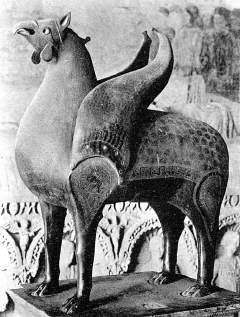
\includegraphics[keepaspectratio=true, width=2.0in]{hippogriff}
  %}
  %\subfigure[A Dragon]{
    %\label{fig:sub:intro:creatures:dragon}
    %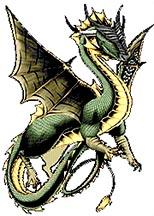
\includegraphics[keepaspectratio=true, width=2.0in]{dragon}
  %}
  \caption{Creatures not drawn using dry erase markers.}
  \label{fig:creatures}
\end{figure}

\section{A Long Section}\label{sec:long}
We need a long chapter to test full-page formatting. Therefore, we
switch to the ancient language of Latin.

%%
% Generated by http://www.lipsum.com
% I could have used the LaTeX package lipsum.sty, but it is not present in all
% LaTeX distributions and would make the examples less portable.
%
Lorem ipsum dolor sit amet, consectetuer adipiscing elit. Maecenas ante augue, dictum ut, scelerisque vitae, sagittis vel, velit. Curabitur velit. Curabitur eleifend eleifend felis. Curabitur purus. Nunc aliquet felis a pede. Suspendisse dictum consequat nunc. In accumsan. Sed sit amet diam. Aliquam rhoncus, orci non sodales suscipit, libero risus condimentum lacus, vitae laoreet velit purus ac est. Etiam id sem eu arcu pellentesque rhoncus. Quisque feugiat est at elit lacinia vestibulum. Integer eget nisl sed diam sodales egestas.

Quisque risus libero, pellentesque ac, iaculis a, pulvinar quis, leo. Cras sapien erat, lacinia sit amet, accumsan porta, bibendum malesuada, nulla. Suspendisse non lorem. Sed pellentesque nulla id nisl. In hac habitasse platea dictumst. Ut nec sem. Proin interdum fringilla felis. Aenean lacus. Quisque nisi. Aliquam congue venenatis purus. Vestibulum ante ipsum primis in faucibus orci luctus et ultrices posuere cubilia Curae; Suspendisse a nunc.

Nunc lobortis. Aliquam ultricies volutpat felis. Nulla nisi tellus, ultrices vel, sodales in, lacinia at, leo. Fusce odio turpis, mattis nec, semper ut, aliquam nec, odio. Sed tristique lacus eget arcu. In at elit. Duis semper, est ut sagittis tempor, risus arcu mattis ligula, quis posuere velit ipsum a neque. Proin mattis, urna vehicula tempus placerat, nisl tortor pharetra dolor, nec luctus orci nisi a ante. Ut a lectus at nulla ultricies congue. Ut rhoncus, purus in malesuada rhoncus, nisi ante laoreet lectus, eget volutpat dui nunc ac metus. Sed dignissim faucibus elit. Vestibulum cursus nonummy mauris. Vestibulum dapibus neque eu ligula. Ut scelerisque urna ut orci tincidunt volutpat. Aliquam ipsum purus, eleifend sed, nonummy non, dapibus vel, metus. Class aptent taciti sociosqu ad litora torquent per conubia nostra, per inceptos hymenaeos.

Ut vitae mauris. Aenean diam. Nam euismod massa bibendum orci. Proin sed arcu. Phasellus commodo lacus. Nunc sit amet dolor eget arcu iaculis congue. Sed volutpat, dolor nec porta facilisis, purus mi euismod lacus, sed pharetra magna arcu id dolor. Vestibulum a purus nec nisl varius facilisis. Sed semper mattis lorem. Suspendisse tellus dolor, tincidunt fermentum, imperdiet eu, ultrices et, massa. Nulla facilisi. Nulla rhoncus. Ut vestibulum quam feugiat quam. Aliquam nisi. Vivamus facilisis euismod ipsum. Nunc suscipit semper felis. Nunc non metus. Vestibulum ante ipsum primis in faucibus orci luctus et ultrices posuere cubilia Curae;

Maecenas posuere rutrum odio. Curabitur dolor quam, semper sed, malesuada eu, sagittis eu, erat. Vestibulum facilisis, ipsum vitae venenatis consectetuer, ipsum nibh scelerisque lacus, quis nonummy elit augue et lectus. Fusce ut dolor et ligula laoreet commodo. Phasellus ornare. Aliquam erat volutpat. Ut sapien leo, auctor vel, placerat vel, pretium quis, libero. Integer tempus interdum tellus. Vestibulum posuere, mi ultricies ullamcorper ornare, dolor nunc condimentum tellus, et commodo neque tellus at mi. Aliquam porttitor, tortor eu interdum malesuada, justo nisl feugiat lacus, eu venenatis augue tortor sit amet arcu. Maecenas quis enim. Mauris fringilla diam. Maecenas vitae metus a felis ullamcorper vestibulum. Suspendisse potenti. Etiam sit amet elit. Ut iaculis risus in odio.

Quisque porttitor, velit at consectetuer pretium, nibh lacus dignissim erat, id imperdiet tellus lectus vel sapien. Integer varius dignissim urna. Vestibulum elementum lobortis lorem. Morbi vel metus in risus consectetuer facilisis. Quisque ac purus eget ipsum interdum semper. Suspendisse blandit, nisi in mattis condimentum, elit sem tempus dui, eu convallis mi dolor in dui. Nunc vehicula eros in diam. Sed lectus velit, varius ut, posuere eget, lacinia a, augue. Suspendisse odio lectus, tincidunt porttitor, porttitor vitae, rhoncus id, turpis. Sed quam. Duis tortor tortor, ultrices ut, imperdiet a, convallis a, magna. Donec pellentesque sapien vitae elit. Fusce egestas eleifend velit. Pellentesque habitant morbi tristique senectus et netus et malesuada fames ac turpis egestas.

Proin ac sapien. Aenean tincidunt ante aliquet tortor. In non elit nec tortor pharetra pretium. Nulla facilisi. Maecenas pulvinar odio in libero. Nam tincidunt nulla et dui. Nunc in eros nec dolor congue varius. Suspendisse euismod. Aliquam nulla nibh, vulputate in, molestie ut, suscipit quis, orci. Ut feugiat sapien id velit. Nullam rutrum, enim non dictum posuere, nulla diam faucibus risus, vel suscipit tellus nisi nec libero. Nullam scelerisque vestibulum sem.

Sed ultrices ligula vel lacus. Donec elit felis, venenatis volutpat, varius eu, placerat cursus, sem. Nullam non felis quis enim laoreet dictum. Nulla in nisl at erat pretium facilisis. Vestibulum sed ante. In hac habitasse platea dictumst. Aenean lobortis ullamcorper ante. Aenean at magna. Etiam viverra erat id augue. Morbi purus. Sed congue. Integer sit amet enim vel sapien ullamcorper auctor. Phasellus neque sapien, cursus sit amet, pharetra ac, mollis non, nibh. Ut risus orci, dignissim eu, feugiat sit amet, ullamcorper sit amet, tortor. Nunc ac ligula ut libero fermentum tincidunt. Morbi lorem metus, bibendum ut, aliquet at, tristique vulputate, nisl. Duis risus turpis, bibendum in, faucibus cursus, eleifend sit amet, erat. Donec elit purus, facilisis nec, vulputate non, gravida et, eros. Curabitur porttitor sapien ac magna. Donec cursus.

Cras sodales posuere pede. Lorem ipsum dolor sit amet, consectetuer adipiscing elit. Donec id nisi eu erat tempus ornare. Ut diam magna, bibendum sit amet, porttitor tempor, malesuada non, tellus. Duis iaculis gravida ante. Morbi dapibus elementum orci. Donec eget metus. Curabitur varius tortor condimentum nunc. In arcu. Nam ante justo, porta sed, pellentesque vitae, tristique in, metus. Nam ultricies nulla quis tellus. Donec egestas enim et dolor. In ornare ligula et eros.

Proin augue ligula, dictum non, viverra vitae, convallis sed, ipsum. Maecenas vitae justo. Lorem ipsum dolor sit amet, consectetuer adipiscing elit. Aliquam erat volutpat. Aenean eget ligula. Nullam id dui eu lacus euismod iaculis. Nulla erat purus, convallis ac, ullamcorper a, vestibulum id, erat. Sed pulvinar consectetuer neque. Nulla lobortis. Nulla congue, sapien in hendrerit rhoncus, est sem dignissim mauris, non nonummy nunc justo volutpat velit. Quisque suscipit risus a ipsum mattis viverra. Pellentesque habitant morbi tristique senectus et netus et malesuada fames ac turpis egestas. Vestibulum ante ipsum primis in faucibus orci luctus et ultrices posuere cubilia Curae; Fusce libero dolor, aliquam vel, varius id, faucibus sollicitudin, massa.

Proin iaculis semper ligula. Pellentesque malesuada, neque sit amet ornare mattis, augue lacus auctor tellus, quis porttitor felis sapien a nibh. In sed orci. Pellentesque congue purus sit amet urna. Proin tincidunt molestie nibh. Nulla et dui ac turpis venenatis ullamcorper. Nunc at nisl. Pellentesque habitant morbi tristique senectus et netus et malesuada fames ac turpis egestas. Cum sociis natoque penatibus et magnis dis parturient montes, nascetur ridiculus mus. Sed magna. Curabitur gravida, metus id semper interdum, dui orci ullamcorper massa, congue ornare mauris lectus rhoncus mi. Integer justo ante, sollicitudin tempor, egestas sit amet, egestas eu, eros. Etiam leo. Integer tristique velit nec nunc.

Nulla ac nibh id nunc volutpat ultrices. Lorem ipsum dolor sit amet, consectetuer adipiscing elit. Praesent a arcu. Suspendisse blandit justo eu justo. Nunc turpis metus, iaculis eget, molestie eu, egestas hendrerit, nibh. Sed elementum placerat metus. Cras pretium turpis non ipsum. Duis in libero. Praesent ut elit eu magna tempus rhoncus. Nunc consectetuer quam ac orci. In nulla.

Donec porta turpis a velit. Donec accumsan. Pellentesque augue magna, cursus sed, elementum eget, cursus id, enim. Duis purus. Suspendisse tristique. Quisque condimentum. Quisque tristique lacus vitae nulla. Nunc nibh velit, gravida et, placerat nec, feugiat sed, ante. Phasellus nisi. Aenean auctor pede at leo. Nullam semper fringilla dui. Quisque est. Suspendisse dolor sem, euismod ac, tempor vitae, nonummy id, felis. Mauris eu tellus. Morbi rhoncus. Cum sociis natoque penatibus et magnis dis parturient montes, nascetur ridiculus mus. Nam sed nisi. Fusce ac sapien sit amet arcu venenatis facilisis. Proin faucibus pharetra risus.

Sed varius elit vitae urna. Ut at felis. Phasellus euismod metus a ante. Suspendisse eu massa. Nullam bibendum dui pulvinar turpis. Mauris lacinia odio id augue. Morbi ligula. Nulla ac massa. Nullam vel arcu. Pellentesque iaculis, tellus et convallis condimentum, erat diam viverra nibh, eget pellentesque mauris lorem faucibus neque.

Curabitur tincidunt, dui ac dictum iaculis, enim magna porttitor orci, quis ullamcorper enim magna commodo justo. Aliquam ut quam in velit porta consequat. Suspendisse potenti. Nunc cursus rutrum eros. Curabitur varius molestie massa. Fusce accumsan fringilla sem. Pellentesque habitant morbi tristique senectus et netus et malesuada fames ac turpis egestas. In hac habitasse platea dictumst. Pellentesque risus nisl, tincidunt sed, sodales ac, interdum ac, diam. In purus ipsum, porttitor feugiat, viverra ac, mattis eget, ligula. Sed bibendum libero in metus. Morbi ornare. Donec libero justo, fringilla vitae, mollis sit amet, molestie ut, mauris. Morbi vel dolor. Donec at elit eget metus semper pharetra. Morbi est massa, volutpat ut, viverra varius, sagittis blandit, sapien. Sed dapibus. Pellentesque erat. Nullam hendrerit. Vestibulum vel diam in tortor consectetuer volutpat.

Quisque accumsan, elit quis sodales pellentesque, sapien metus consequat enim, et commodo leo nulla in elit. Donec varius. Donec ut risus. Donec quis lacus quis nisi congue consectetuer. In sed odio. Duis nulla sem, ullamcorper ac, suscipit dignissim, suscipit vel, turpis. Fusce suscipit. Maecenas in augue non felis fermentum luctus. Aenean sem. Etiam in leo sit amet tortor malesuada auctor. Curabitur quis massa. Maecenas aliquam lectus. Maecenas sit amet augue. Sed sem elit, egestas vitae, condimentum suscipit, elementum et, nulla. Lorem ipsum dolor sit amet, consectetuer adipiscing elit. Nam dignissim tristique velit.

Pellentesque dui elit, tristique non, cursus a, elementum sed, magna. Ut eu augue. Maecenas scelerisque lectus vel enim. Vivamus eu mauris. Phasellus venenatis. Maecenas egestas. Phasellus ac purus. Sed vel dui. Nam consectetuer venenatis lacus. Morbi ullamcorper, urna ac viverra tempor, urna dui imperdiet dui, sit amet hendrerit elit nisi ac lorem. Nullam gravida diam ut tellus. Aenean quam tortor, condimentum ac, commodo non, pharetra in, elit. Mauris tincidunt, orci sit amet lacinia varius, diam tortor dapibus tellus, id scelerisque quam magna pharetra libero. Curabitur aliquet, ante sit amet ornare volutpat, urna ipsum dictum ipsum, at ullamcorper ligula arcu eget leo.

Ut libero lorem, condimentum nec, rhoncus id, vestibulum a, nisl. Cras hendrerit euismod sapien. Sed lectus ipsum, vehicula et, luctus vitae, venenatis at, magna. Ut nec nisl in quam facilisis tincidunt. Fusce enim purus, pellentesque vitae, molestie ut, dapibus in, eros. Integer eu turpis vel pede volutpat posuere. Nam porttitor suscipit metus. Curabitur mollis, quam quis porttitor nonummy, libero ante pulvinar magna, a bibendum massa erat nec sapien. Donec ac turpis. Suspendisse elit nisi, ultrices ut, fringilla sed, vestibulum suscipit, mauris. Cum sociis natoque penatibus et magnis dis parturient montes, nascetur ridiculus mus. Phasellus dictum aliquam lacus. Praesent in erat quis nunc consectetuer dictum. Morbi dignissim, turpis ut varius pharetra, tellus lectus rutrum lacus, bibendum iaculis velit nulla ac orci. Etiam gravida nibh eget massa. Sed elementum convallis purus. Duis tincidunt feugiat lacus. Donec id enim nec enim ullamcorper condimentum. Suspendisse urna.


\section{Conclusions}
Of course, no report would be complete without some conclusions.
This section is where they would go, if we had some.

% I've never used the following 3 commands but maybe you will
\initials{ H.P. }

%\enc{   }

\keywords{ Dry erase markers }

\nocite{*}

% ---------------------------------------------------------------------- %
% References
%
\normalfont 
\bibliographystyle{plain}
\bibliography{SANDExample}

% ---------------------------------------------------------------------- %
% Appendices
% 
\clearpage
\renewcommand{\thesection}{\Alph{section}}
\setcounter{section}{0}

\section{Historical Perspective}
This is an example of an appendix.

\subsection{The Past a Long Time Ago}
This is where we talk about things so old nobody can verify them. We
are safe. 

\subsection{The Past More Recently}
Now we have to be a little bit more careful, since records exist from
that time, and some people still alive actually lived back then.

\section{Some Other Appendix}
Just to show what a second Appendix would look like. It contains
a table. 

\begin{table}[ht]
  \centering
  \caption{A small table}
  \bigskip
  
  \begin{tabular}{|c|c|}
    \hline
    A & B  \\ \hline
    C & D  \\ \hline
  \end{tabular}
  \label{tab3}
\end{table}

\begin{figure}[ht]
  \centering
  \begin{picture}(50,50)(0,0)
    \put(25,25){\circle{1}}
    \put(25,25){\circle{5}}
    \put(25,25){\circle{10}}
    \put(25,25){\circle{15}}
    \put(25,25){\circle{20}}
    \put(25,25){\circle{25}}
    \put(25,25){\circle{30}}
    \put(25,25){\circle{35}}
    \put(25,25){\circle{40}}
    \put(25,25){\circle{45}}
    \put(25,25){\circle{50}}
  \end{picture}
  \caption{Dizzy yet?}
  \label{fig4}
\end{figure}

% ---------------------------------------------------------------------- %
% Distribution list
% 
\clearpage
\begin{distribution}{External Distribution:}
    \normalfont
    An Address\\
    99 $99^{th}$ street NW\\
    City, State\\
    \\
    Some Address\\
    and street\\
    City, State\\
    \\
    Another Address\\
    On a street\\
    City, State\\
    U.S.A.
\end{distribution}

\begin{distribution}{Internal Distribution:}
    \normalfont
    \begin{tabular}{@{}lll}
	MS-1319 & R. E. Riesen & Org. 1423\\[3pt]
	MS-1234 & A. Nother & Org. 4321
    \end{tabular}
\end{distribution}

% ---------------------------------------------------------------------- %
% End
% 
\end{memo}

\end{document}
